
\section{Les structures de données}
\subsection{Les enregistrements}

\begin{frame}
	\begin{center}
		\huge  Les structures de données
		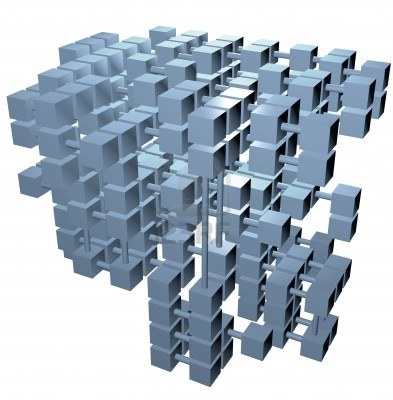
\includegraphics[scale=0.6]{pics/struct.jpg}
	\end{center}
\end{frame}


\begin{frame}[fragile]
	\frametitle{Enregistrements}
	\begin{itemize}
	\item Déclaration de type: 
		\begin{lstlisting}
		type pixel = 
		{ mutable  r:int ; mutable g:string 
		; b:int } 
		\end{lstlisting}
		Un champ mutable signifie qu'il peut être modifié.
	
	\item Modifiaction des champs de valeur:
		\begin{lstlisting}
			p.r <- 42.0;
			p.g <- "The Game"
		\end{lstlisting}
\end{itemize}
\end{frame}


\begin{frame}[fragile]
	\frametitle{Les références}
	Une référence est considéré comme l'équivalent (selon l'INRIA) des pointeurs en OCaml.
	\begin{lstlisting}
		type 'a ref = {mutable contents:'a}
	\end{lstlisting}
	Déclaration:
	\begin{lstlisting}
		let a = ref 0

		let l = ref [];;
		val l : '_a list ref = {contents=[]}
	\end{lstlisting}
	Utilisation:
	\begin{lstlisting}
		!a ;;
		- : int = 0
		a := !a + 1 ;;
		- : unit = ()
	\end{lstlisting}

\end{frame}

\subsection{Les vecteurs}

\begin{frame}
	\frametitle{Les vecteurs}
	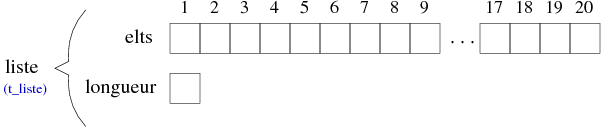
\includegraphics[scale=0.5]{pics/vect.png}
\end{frame}

\begin{frame}[fragile]
	\frametitle{Les vecteurs}
	\framesubtitle{Création}
	\begin{itemize}
	\item
	\begin{lstlisting}
	let v = [| 3.14; 6.28; 9.42 |];;
	val v : float array = [|3.14; 6.28; 9.42|]
	\end{lstlisting}

	\item Array.create
	\begin{lstlisting}
	let v = Array.create  3  3.14;;
	val v : float array = [|3.14; 3.14; 3.14|]
	\end{lstlisting}

	\item Array.make
	\end{itemize}
\end{frame}


\begin{frame}[fragile]
	\frametitle{Les vecteurs}
	\framesubtitle{Utilisation simple}
	\begin{enumerate}
	\item
	\begin{lstlisting}
	v.(1) ;;
	- : float = 3.14
	\end{lstlisting}

	\item
	\begin{lstlisting}
	v.(0) <- 100.0 ;;
	- : unit = ()
	\end{lstlisting}

	\item
	\begin{lstlisting}
	v ;;
	- : float array = [|100; 3.14; 3.14|]
	\end{lstlisting}
	\end{enumerate}
\end{frame}

\begin{frame}[fragile]
	\frametitle{The Game}
	\framesubtitle{Vecteur(ception)}
	\begin{lstlisting}
	let t = [| 
           [|1|];
           [|1; 1|];
           [|1; 2; 1|];
           [|1; 3; 3; 1|];
           [|1; 4; 6; 4; 1|];
           [|1; 5; 10; 10; 5; 1|]
         |] 
	\end{lstlisting}
\end{frame}

\begin{frame}[fragile]
	\frametitle{Les vecteurs}
	\framesubtitle{Copie et valeurs partagées}
	\begin{lstlisting}
	let v2 = Array.copy v ;;
	val v2 : int array = [|1; 0; 0|]
	let m2 = Array.copy m ;;
	val m2 : int array array = 
	[|[|1; 0; 0|]; [|1; 0; 0|]; [|1; 0; 0|]|]

	v.(1)<- 1337;;
	- : unit = ()

	v2;; 
	- : int array = [|1; 0; 0|]
	m2 ;;
	- : int array array = 
	[|[|1; 1337; 0|]; [|1; 1337; 0|]; 
	[|1; 1337; 0|]|]
	\end{lstlisting}
\end{frame}

\begin{frame}[fragile]
	\frametitle{Les vecteurs}
	\framesubtitle{Autres fonctionnalitées du module Array}
	\begin{itemize}
	\item Array.make\_matrix
	
	\item Array.sub (Ex: Array.sub a start n)
	
	\item Array.\{iter,map,iteri,to\_list\}

	\item RTFM !!!
	\end{itemize}
\end{frame}


\begin{frame}
	\frametitle{Les piles}
	
\includegraphics[scale=0.4]{pics/stack.jpg}
\end{frame}

\begin{frame}[fragile]
	\frametitle{Les piles}
	\framesubtitle{Initialisation}
	Pour utiliser les piles en OCaml nous vous présenterons ici le module Stack (ensuite si ça vous amuse de les recoder...):
	\begin{lstlisting}
	open Stack
	\end{lstlisting}
	Pour créer une pile on utilise:
	\begin{lstlisting}
	let s = Stack.create ();;
	val s : '_a Stack.t = <abstr>
	\end{lstlisting}
\end{frame}

\subsection{Les piles}
\begin{frame}[fragile]
\frametitle{Les piles}
\framesubtitle{Utilisation}
	\begin{itemize}
	
	\item
		\begin{lstlisting}
		Stack.push "42" s; Stack.push s "1337";;
		- : unit = ()	
		\end{lstlisting}	
	
	\item
		\begin{lstlisting}
		Stack.pop s;;
		- : string = "43"
		Stack.top s;;
		- : string = "42"
		\end{lstlisting}	

	\end{itemize}

\end{frame}

\begin{frame}[fragile]
\frametitle{Les piles}
\framesubtitle{Les fonctions essentielles}
	\begin{itemize}
	
	\item
		\begin{lstlisting}
		Stack.clear
		\end{lstlisting}

	\item
		\begin{lstlisting}
		Stack.copy
		\end{lstlisting}	

	\item
		\begin{lstlisting}
		Stack.is_empty
		\end{lstlisting}	

	\item
		\begin{lstlisting}
		Stack.length
		\end{lstlisting}	

	\item
		\begin{lstlisting}
		Stack.iter
		\end{lstlisting}

	\end{itemize}

\end{frame}

\begin{frame}
	\frametitle{Les tables de hachage}
	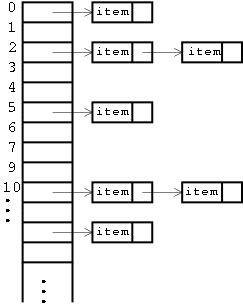
\includegraphics[scale=0.6]{pics/hash.jpg}
\end{frame}

\subsection{Les tables de hachage}
\begin{frame}[fragile]
\frametitle{Les tables de hachage}
\framesubtitle{Initialisation}
	Ici seront présentée les tables de hachage du module Hashtbl (qui fais du hachage dynamique
	\begin{lstlisting}
	open Hashtbl
	\end{lstlisting}
	Pour créer une pile on utilise:
	\begin{lstlisting}
	Hashtbl.create
	val create : ?random:bool -> int -> ('a, 'b) t
	\end{lstlisting}
\end{frame}

\begin{frame}[fragile]
\frametitle{Les tables de hachage}
\framesubtitle{Utilisation}
	\begin{itemize}
	
	\item
		\begin{lstlisting}
		Hashtbl.add   VS   Hashtbl.replace
		\end{lstlisting}	
	
	\item
		\begin{lstlisting}
		Hashtbl.remove h x
		Hashtbl.find h x
		Hashtbl.find_all h x
		\end{lstlisting}	

	\end{itemize}


\end{frame}

\begin{frame}[fragile]
\frametitle{Les tables de hachage}
\framesubtitle{Les fonctions essentielles}
	\begin{itemize}
	
	\item
		\begin{lstlisting}
		Hashtbl.clear
		\end{lstlisting}

	\item
		\begin{lstlisting}
		Hashtbl.copy
		\end{lstlisting}	

	\item
		\begin{lstlisting}
		Hashtbl.mem
		\end{lstlisting}	

	\item
		\begin{lstlisting}
		Hashtbl.length
		\end{lstlisting}

	\end{itemize}

\end{frame}

